\documentclass[10pt]{article}
\usepackage[paperwidth=12in,paperheight=4.8in,margin=0.22in]{geometry}
\usepackage{amsmath,amssymb}
\usepackage{xcolor}
\usepackage{tikz}
\usetikzlibrary{positioning}
\usepackage[scaled=0.96]{helvet}
\renewcommand{\familydefault}{\sfdefault}
\pagestyle{empty}
\setlength{\parindent}{0pt}

\definecolor{Navy}{HTML}{17234D}
\definecolor{Blue}{HTML}{087EBA}
\definecolor{PaleBlue}{HTML}{EAF3F8}
\definecolor{PaleGray}{HTML}{F1F3F5}
\definecolor{Orange}{HTML}{E97828}

\begin{document}
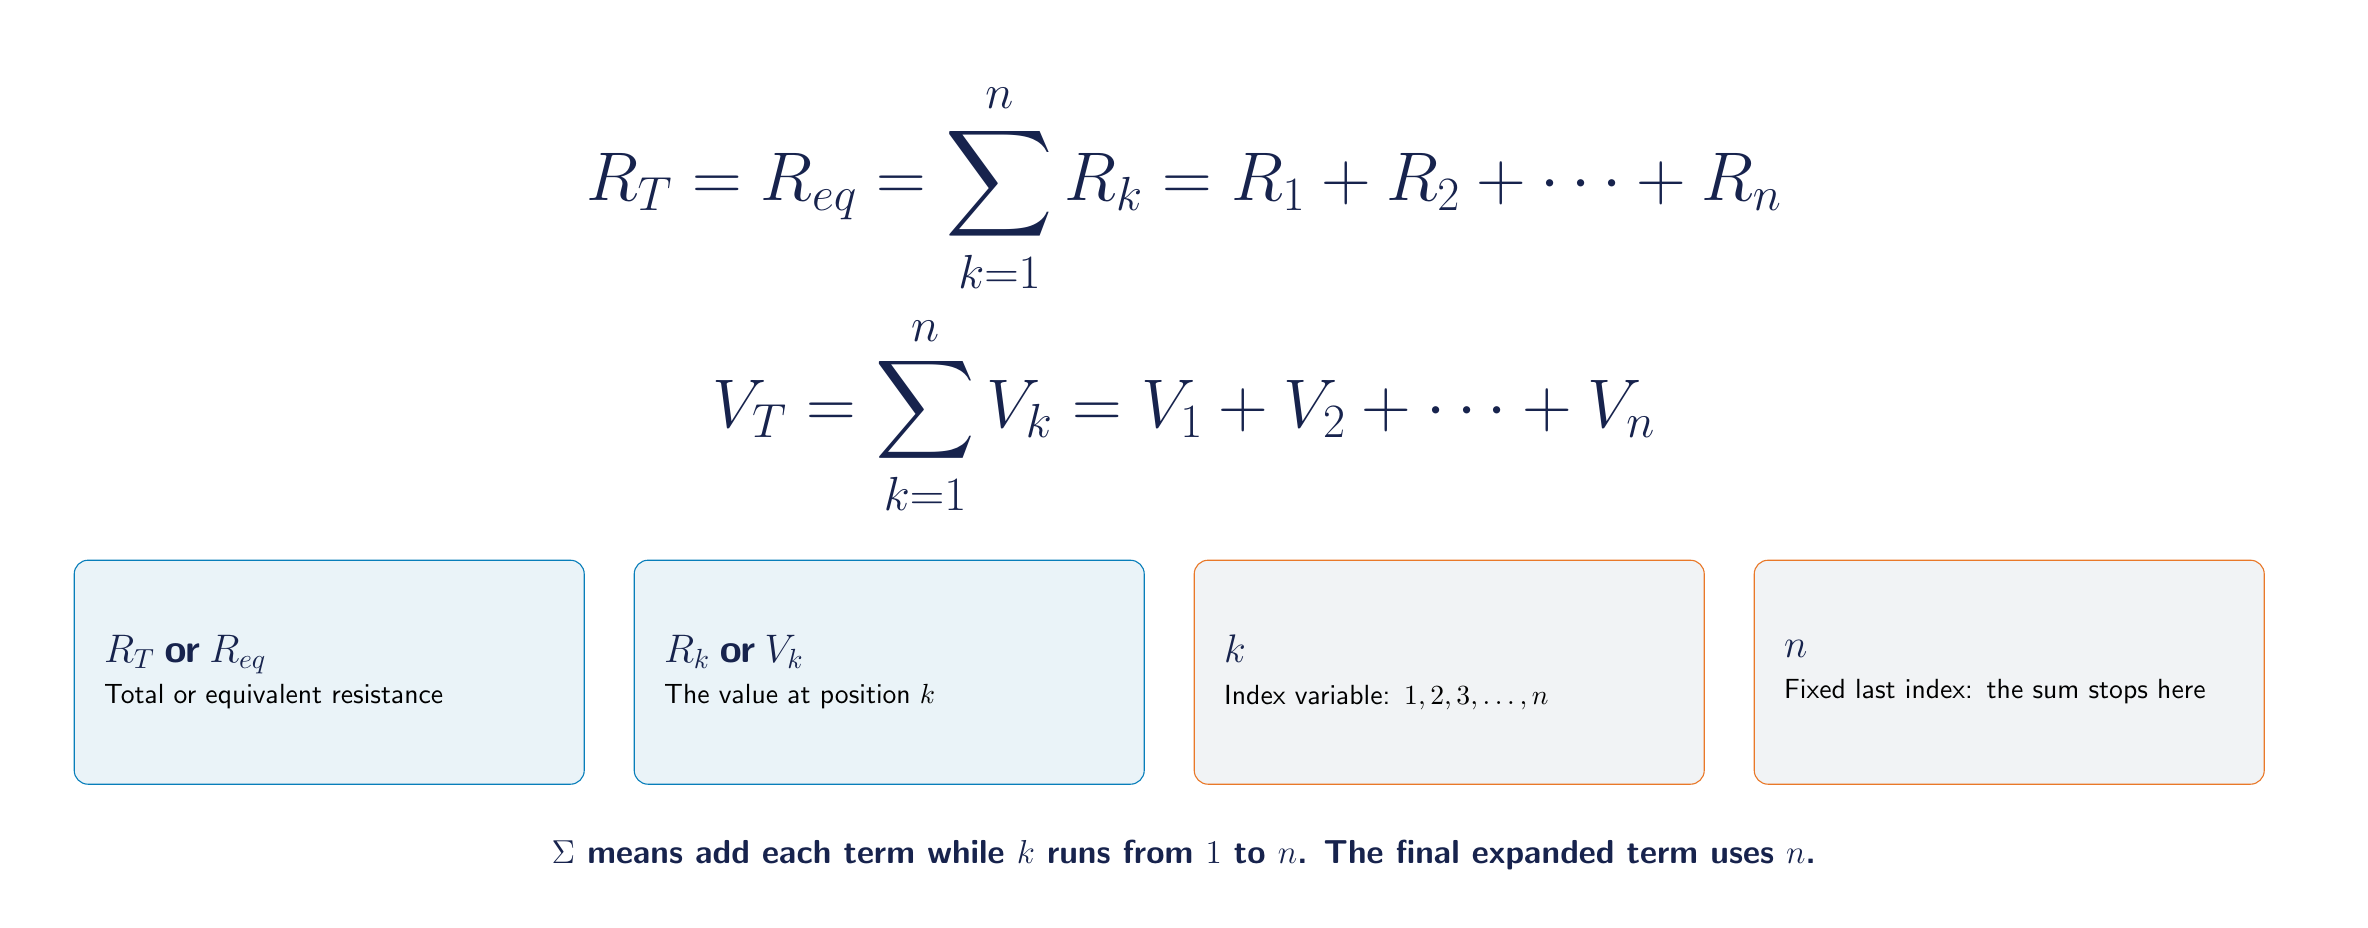
\begin{tikzpicture}[x=1in,y=1in]
  \useasboundingbox (0,0) rectangle (11.56,4.36);
  \fill[white] (0,0) rectangle (11.56,4.36);

  \node[anchor=north west,inner sep=0] at (0.13,4.25) {
    \begin{minipage}{11.3in}
      \centering
      {\color{Navy}\fontsize{27}{32}\selectfont
      \[
        R_T=R_{eq}=\sum_{k=1}^{n}R_k
        =R_1+R_2+\cdots+R_n
      \]}
      \vspace{-0.08in}
      {\color{Navy}\fontsize{25}{30}\selectfont
      \[
        V_T=\sum_{k=1}^{n}V_k
        =V_1+V_2+\cdots+V_n
      \]}
    \end{minipage}
  };

  \node[draw=Blue,fill=PaleBlue,rounded corners=5pt,minimum width=2.55in,minimum height=1.12in,align=left,anchor=north west,text width=2.25in] at (0.23,1.70) {
    {\color{Navy}\Large\bfseries $R_T$ or $R_{eq}$}\\[3pt]
    Total or equivalent resistance
  };

  \node[draw=Blue,fill=PaleBlue,rounded corners=5pt,minimum width=2.55in,minimum height=1.12in,align=left,anchor=north west,text width=2.25in] at (3.03,1.70) {
    {\color{Navy}\Large\bfseries $R_k$ or $V_k$}\\[3pt]
    The value at position $k$
  };

  \node[draw=Orange,fill=PaleGray,rounded corners=5pt,minimum width=2.55in,minimum height=1.12in,align=left,anchor=north west,text width=2.25in] at (5.83,1.70) {
    {\color{Navy}\Large\bfseries $k$}\\[3pt]
    Index variable: $1,2,3,\ldots,n$
  };

  \node[draw=Orange,fill=PaleGray,rounded corners=5pt,minimum width=2.55in,minimum height=1.12in,align=left,anchor=north west,text width=2.25in] at (8.63,1.70) {
    {\color{Navy}\Large\bfseries $n$}\\[3pt]
    Fixed last index: the sum stops here
  };

  \node[anchor=south,color=Navy,font=\bfseries\large] at (5.78,0.10) {$\Sigma$ means add each term while $k$ runs from $1$ to $n$. The final expanded term uses $n$.};
\end{tikzpicture}
\end{document}

